%%%%%%%%%%%%%%%%%%%%%%%%%%%%%%%%%%%%%%%%%
% Beamer Presentation
% LaTeX Template
% Version 1.0 (10/11/12)
%
% This template has been downloaded from:
% http://www.LaTeXTemplates.com
%
% License:
% CC BY-NC-SA 3.0 (http://creativecommons.org/licenses/by-nc-sa/3.0/)
%
%%%%%%%%%%%%%%%%%%%%%%%%%%%%%%%%%%%%%%%%%

%----------------------------------------------------------------------------------------
%	PACKAGES AND THEMES
%----------------------------------------------------------------------------------------

\documentclass{beamer}
%\usepackage{cite}

\mode<presentation> {

% The Beamer class comes with a number of default slide themes
% which change the colors and layouts of slides. Below this is a list
% of all the themes, uncomment each in turn to see what they look like.

%\usetheme{default}
%\usetheme{AnnArbor}
%\usetheme{Antibes}
%\usetheme{Bergen}
%\usetheme{Berkeley}
%\usetheme{Berlin}
%\usetheme{Boadilla}
%\usetheme{CambridgeUS}
%\usetheme{Copenhagen}
%\usetheme{Darmstadt}
%\usetheme{Dresden}
%\usetheme{Frankfurt}
%\usetheme{Goettingen}
%\usetheme{Hannover}
%\usetheme{Ilmenau}
%\usetheme{JuanLesPins}
%\usetheme{Luebeck}
\usetheme{Madrid}
%\usetheme{Malmoe}
%\usetheme{Marburg}
%\usetheme{Montpellier}
%\usetheme{PaloAlto}
%\usetheme{Pittsburgh}
%\usetheme{Rochester}
%\usetheme{Singapore}
%\usetheme{Szeged}
%\usetheme{Warsaw}

% As well as themes, the Beamer class has a number of color themes
% for any slide theme. Uncomment each of these in turn to see how it
% changes the colors of your current slide theme.

%\usecolortheme{albatross}
%\usecolortheme{beaver}
%\usecolortheme{beetle}
%\usecolortheme{crane}
%\usecolortheme{dolphin}
%\usecolortheme{dove}
%\usecolortheme{fly}
%\usecolortheme{lily}
%\usecolortheme{orchid}
%\usecolortheme{rose}
%\usecolortheme{seagull}
%\usecolortheme{seahorse}
%\usecolortheme{whale}
%\usecolortheme{wolverine}

%\setbeamertemplate{footline} % To remove the footer line in all slides uncomment this line
%\setbeamertemplate{footline}[page number] % To replace the footer line in all slides with a simple slide count uncomment this line

%\setbeamertemplate{navigation symbols}{} % To remove the navigation symbols from the bottom of all slides uncomment this line
}

\usepackage{media9}
\usepackage{graphicx} % Allows including images
\usepackage{booktabs} % Allows the use of \toprule, \midrule and \bottomrule in tables
\usepackage{parskip}
\usepackage{caption}
\usepackage{subcaption}
\usepackage{tikz}
\usepackage{multicol}
\renewcommand{\arraystretch}{1.5}
%\usepackage{cite}



%----------------------------------------------------------------------------------------
%	TITLE PAGE
%----------------------------------------------------------------------------------------

\title[Indaba 2017]{Experience at the Deep Learning Indaba 2017} % The short title appears at the bottom of every slide, the full title is only on the title page


\author{Alice Nanyanzi} % Your name
\institute{} % Your institution as it will appear on the bottom of every slide, may be shorthand to save space

\date{August 24, 2017} % Date, can be changed to a custom date


\begin{document}

\begin{frame}[noframenumbering, plain]
\titlepage % Print the title page as the first slide
\end{frame}

\begin{frame}{The Indaba, First of it's kind}
		\begin{figure}
		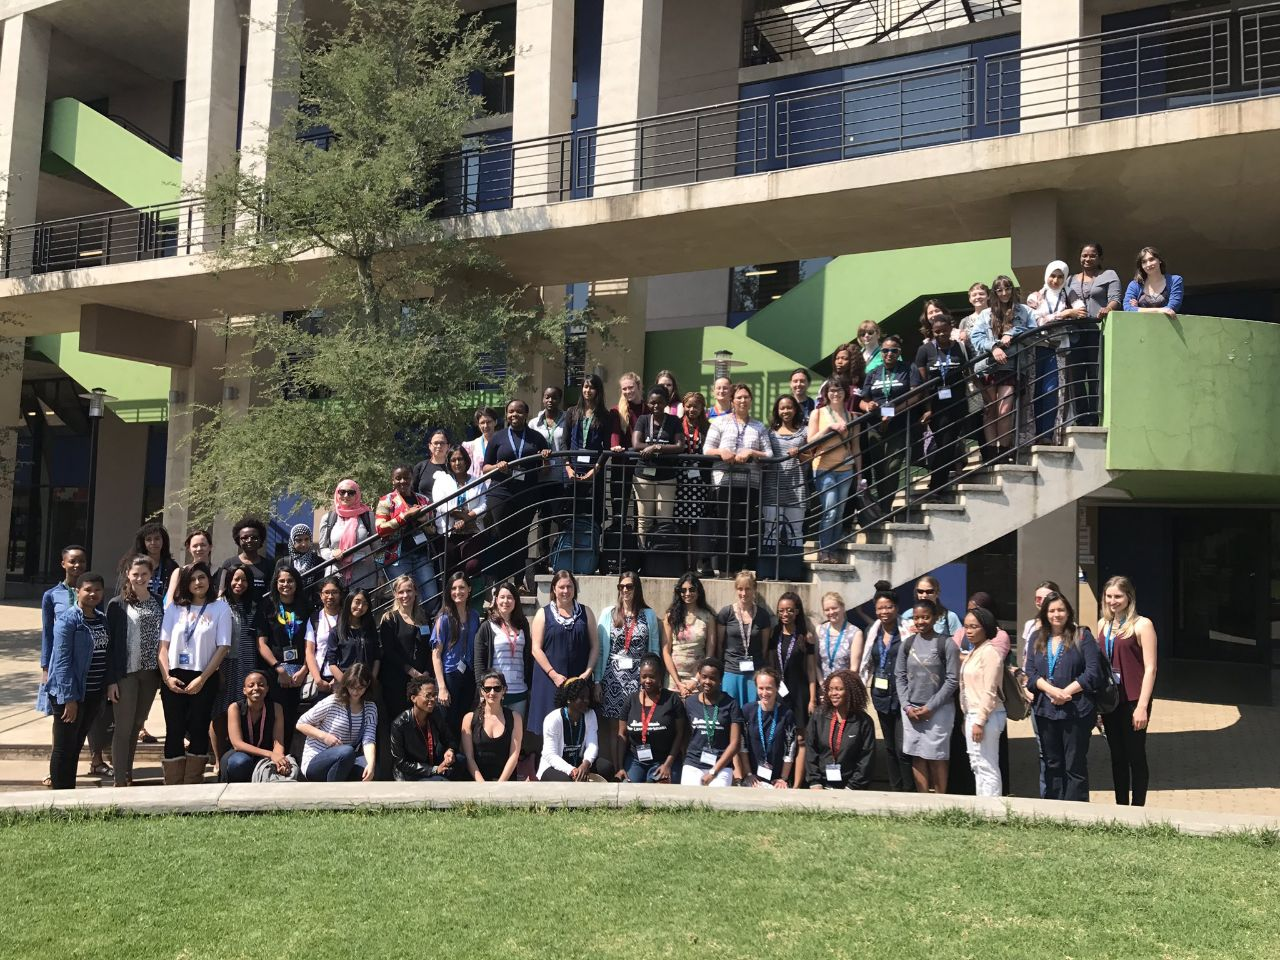
\includegraphics[width=0.65\textwidth]{indabafemale.jpg}
		\caption{ Women Participants}
	\end{figure}
	
\end{frame}

\begin{frame}{Events and Network Forums}
	
	\begin{itemize}[<+->]
	\item Machine Learning and Data Science in Africa network forum\\
	A mailing list for updates, collaborations, etc
	\item Women in machine learning workshop \url{http://wimlworkshop.org/2017/}
	
	\item Black in AI workshop 
	\url{https://ai.stanford.edu/~tgebru/blackAI}
	\end{itemize} 
	
\end{frame}
\begin{frame}{Exhibitions}		
	\begin{figure}
		\begin{subfigure}[b]{0.40\textwidth}
				
\includegraphics[width=\textwidth]{opti-num.png}
		\end{subfigure}~
	     \hspace*{2cm}
		\begin{subfigure}[b]{0.30\textwidth}
				
\includegraphics[width=\textwidth]{retrorabbit.png}
		\end{subfigure}\\
	    \vspace*{2cm}
	    \begin{subfigure}[b]{0.35\textwidth}
		
\includegraphics[width=\textwidth]{standardbank.jpg}
	    \end{subfigure}~
       \hspace*{2cm}
	   \begin{subfigure}[b]{0.35\textwidth}
			    	
\includegraphics[width=\textwidth]{ibmlogo.jpg}
	   \end{subfigure}
	   
	\end{figure}
\end{frame}

\begin{frame}{Visit at Google offices, Johannesburg}	
	\begin{figure}[!h]
		\centering	
			\only<1->{\includegraphics<1>[scale=0.7]{reception.jpeg}}
			\only<2->{\includegraphics<2>[width=0.50\textwidth]{Google-ZA-canteen.jpg}}
			\only<3->{\includegraphics<3>[width=0.50\textwidth]{Google-ZA-meeting-room-wall-decorations-sound-dampeners.jpg}}
			\caption{\only<1>{Google Reception}\only<2>{The Canteen} \only<3>{Meeting Area} }
	\end{figure}	
	
\end{frame}

\begin{frame}{Panel Discussion}
	\begin{itemize}
		\item Identifying potential supervisors
		\item Writing papers
		\item Research Experience of the panelists
	\end{itemize}
\end{frame}


\begin{frame}{IBM Research Lab Visit}
	\begin{figure}
		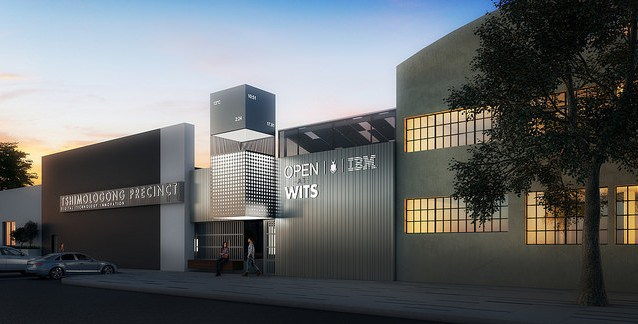
\includegraphics[width=0.8\textwidth]{ibmafrica.jpg}
		\caption{ IBM Research Lab Johannesberg (Tshimologong Precinct)}
	\end{figure}
\end{frame}

\begin{frame}{ Research at IBM Research Lab}
	\begin{itemize}
	\item Personalised learning
	\item Exploring the universe
	\item Digital Urban Ecosystems
	\item[\textcolor{red}{\textbullet}] Data Driven healthcare	
	\end{itemize}
	\begin{figure}
	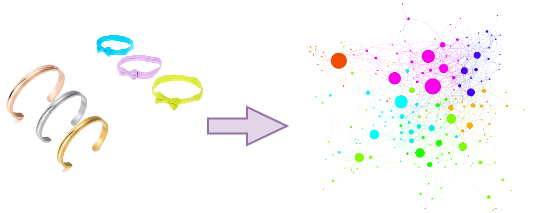
\includegraphics[width=0.8\textwidth]{tb.png}
	\caption{Track TB spread through Fashion Wearables}
	\end{figure}

\end{frame}




\end{document} 